\documentclass[xcolor={dvipsnames}]{beamer}
\usetheme{Malmoe}
\usecolortheme{spruce}
\setbeamercolor{item}{fg=PineGreen}
\setbeamertemplate{itemize item}[square]
\setbeamertemplate{itemize subitem}[triangle]
\setbeamertemplate{itemize subsubitem}[square]
\setbeamertemplate{itemize/enumerate subbody begin}{\vspace{0.5em}}
\setbeamercolor*{bibliography entry title}{fg=black}
\setbeamercolor*{bibliography entry author}{fg=black}
\setbeamercolor*{bibliography entry location}{fg=black}
\setbeamercolor*{bibliography entry note}{fg=black}
% and kill the abominable icon
\setbeamertemplate{bibliography item}{}

\usepackage{natbib}
\usepackage{amsmath,amsthm,amssymb}
\usepackage{mathtools}
\usepackage{mathrsfs}
\usepackage{bm}
\usepackage{physics}
\usepackage{slashed}
\usepackage{graphicx}
\usepackage{caption}

\captionsetup[figure]{labelformat=empty}
\graphicspath{ {./images/} }

\let\olditemize=\itemize 
\let\endolditemize=\enditemize 
\renewenvironment{itemize}{\olditemize \itemsep=.5em }{\endolditemize}

\title{Quantum Hadrodynamics}
\subtitle{From Fundamental Fields to Nuclear Phenomena}
\author{Sean Ericson}
\institute{UO\\PHYS 663}
\date{June 13, 2024}
\titlegraphic{\includegraphics[scale=0.6]{seal.jpg}}

\begin{document}

\frame{\titlepage}

\begin{frame}{A Brief History of Nuclear Physics}
\alert{From Plumb Pudding to Nuclear Apocalypse}
\begin{itemize}
    \item<2-> 1904: J.J. Thompson proposes plumb pudding model of atoms after discovering electrons in 1897.
    \item<3-> 1911-1917: Rutherford discovers nucleus, proton.
    \item<4-> 1935: Chadwick discovers neutron.
    \item<5-> 1942: Fermi, first successful reactor (CP-1).
    \item<6-> 1945: Trinity test
    \item<7-> 2023: BARBENHEIMER
\end{itemize}
\end{frame} 

\begin{frame}
    \begin{figure}
        \centering
        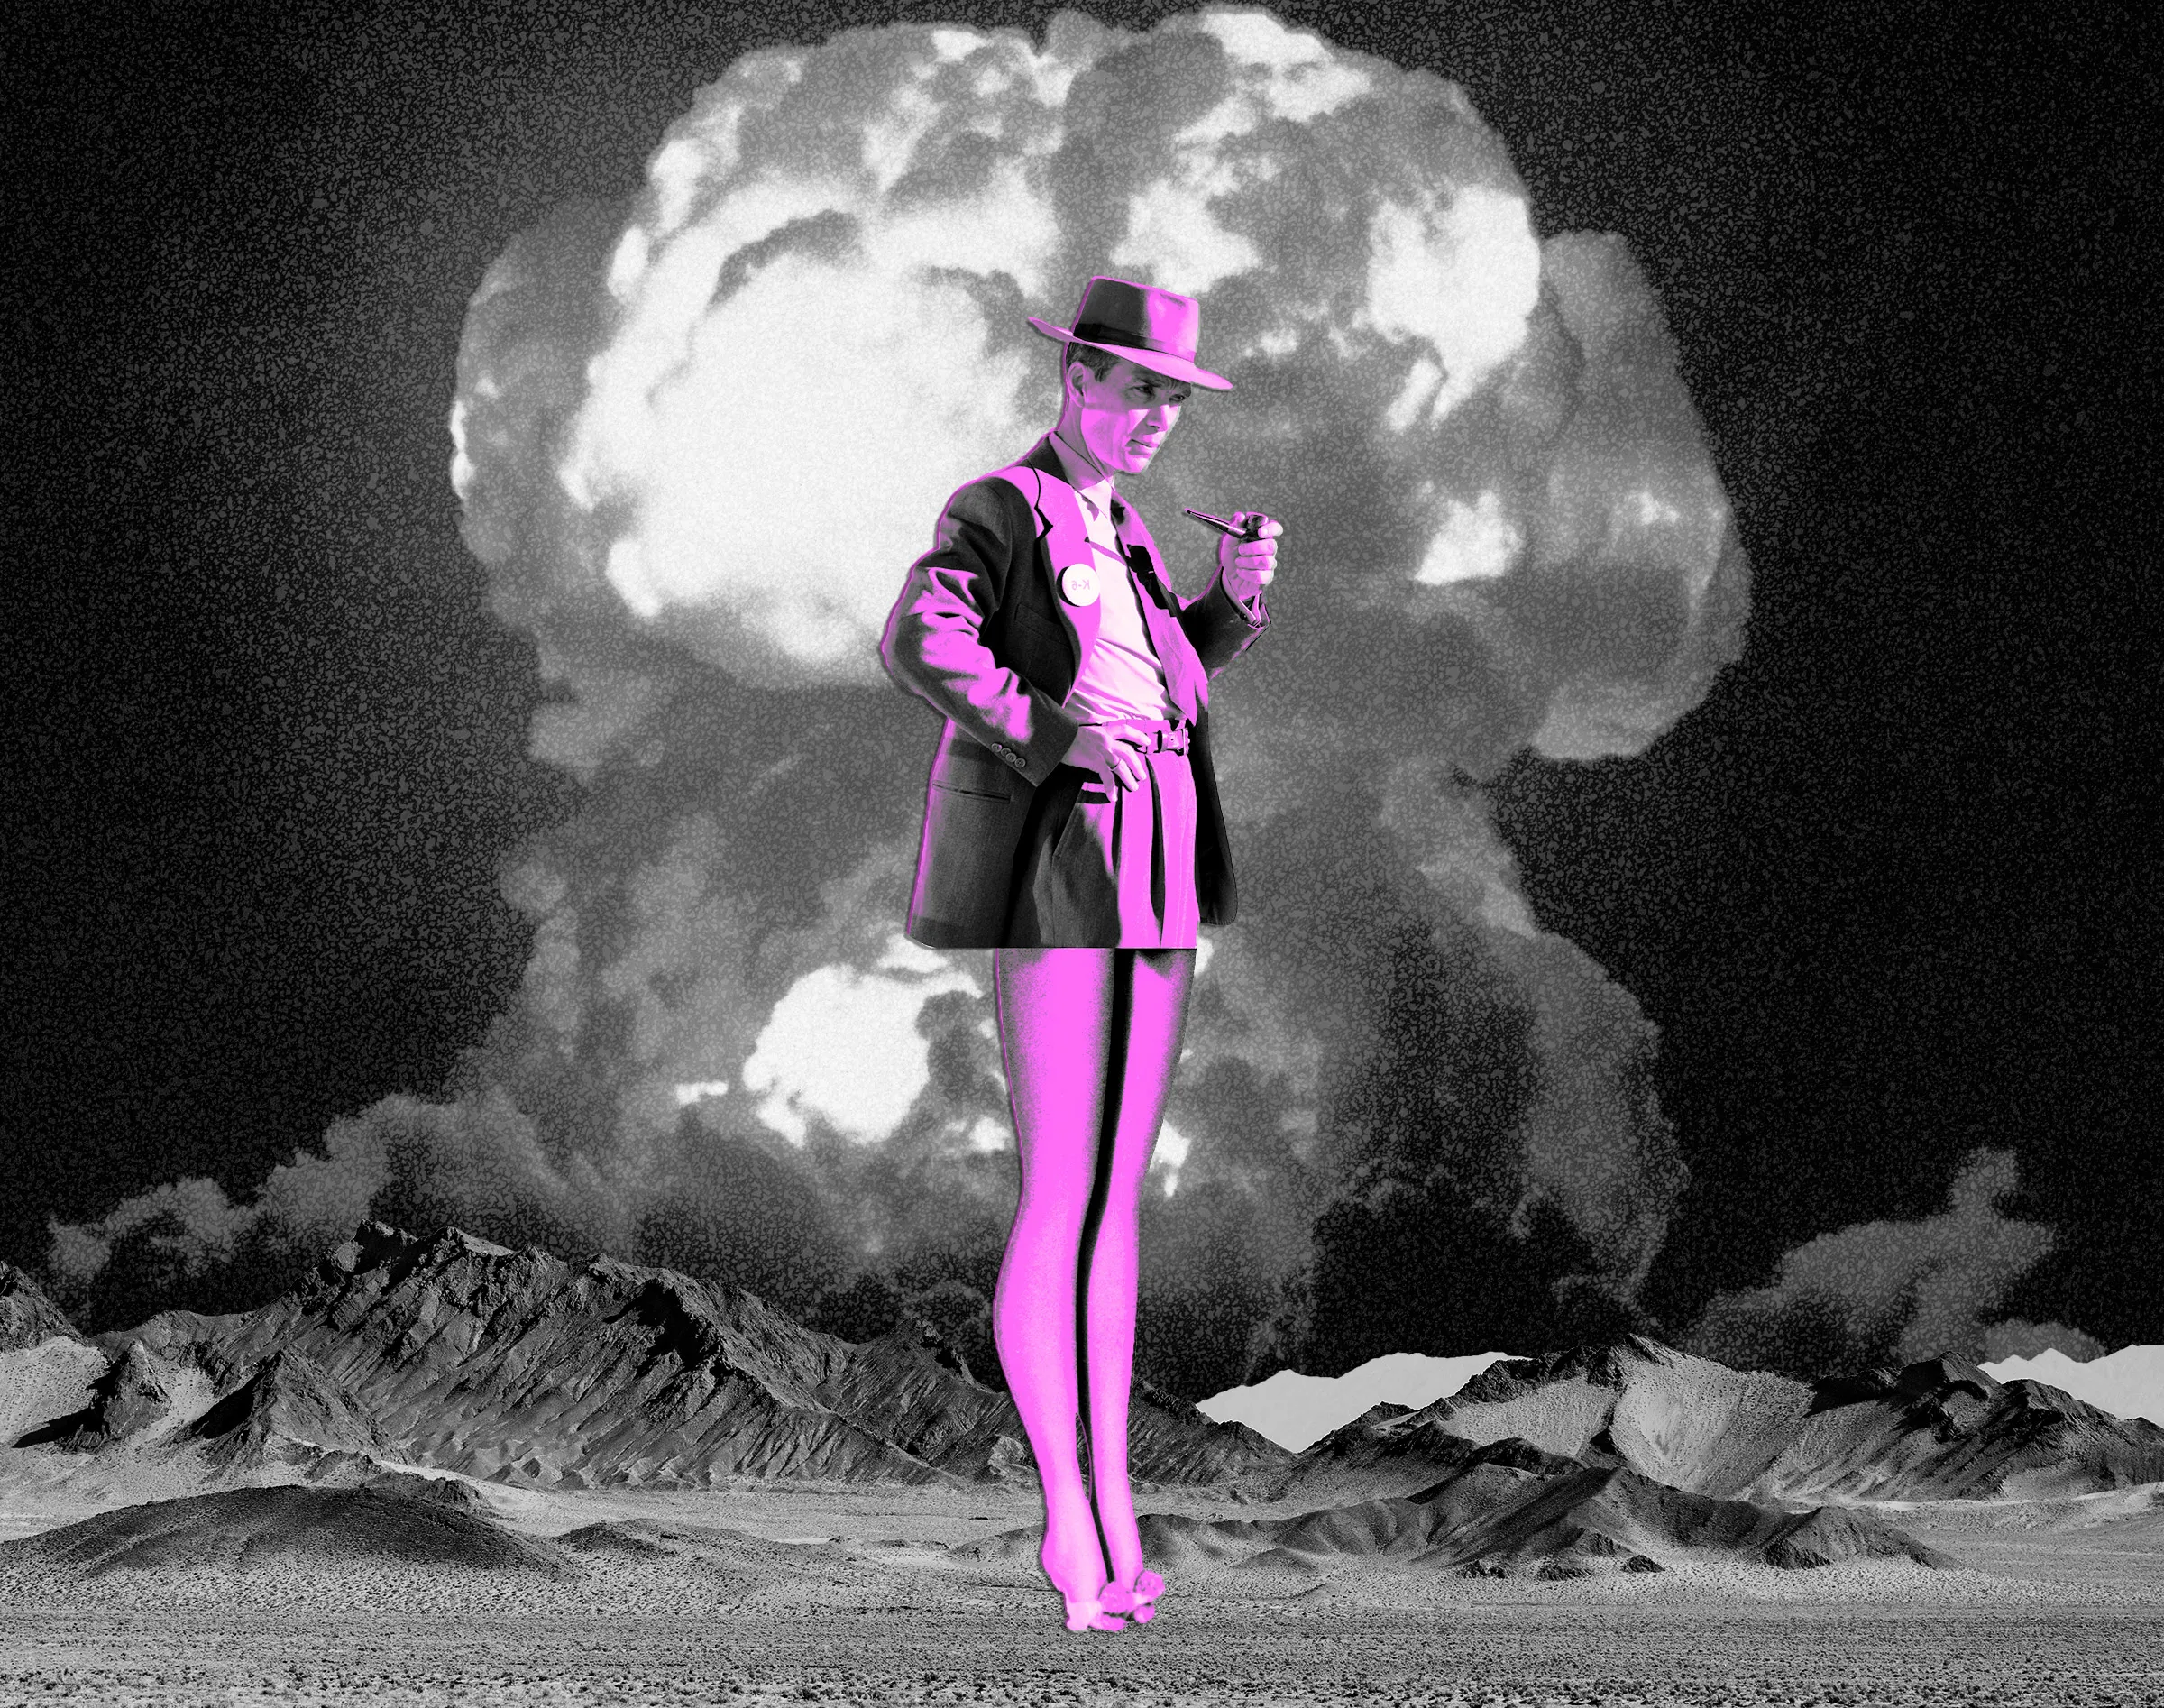
\includegraphics[scale=0.27]{barbenheimer.png}
    \end{figure}
\end{frame}

\begin{frame}{A Brief Intro to Nuclear Physics}
\alert{Iso-what now??}
\begin{itemize}
    \item<2-> Nucleons
    \begin{itemize}
        \item<3-> $m_p \approx 938.272$ MeV
        \item<4-> $m_n \approx 939.565$ MeV
        \item<5-> $\Delta m / m_p \approx 0.14\%$
    \end{itemize}
    \item<6-> Nuclei
    \begin{itemize}
        \item<7-> $Z$: \# of protons ($Z_1  = Z_2 \implies$ ``isotopes'')
        \item<8-> $N$: \# of neutrons ($N_1 = N_2 \implies$ ``isotones'')
        \item<9-> $A = Z + N$: Total \# of nucleons ($A_1 = A_2 \implies$ ``isobars'')
    \end{itemize}
    \item<10-> Iso(baric)spin
    \begin{itemize}
        \item<11-> $p$, $n$ are just two different ``isospin charge'' states of the nucleon
        \item<12-> $p = \ket{\frac{1}{2}, \frac{1}{2}}$, $n = \ket{\frac{1}{2}, -\frac{1}{2}}$; $\pi^\pm = \ket{1, \pm 1}$, $\pi^0 = \ket{1, 0}$
    \end{itemize}
\end{itemize}
\end{frame}

\begin{frame}{${}^2D$: The Simplest Nucleus}
\alert{Well, besides ${}^1H$}
\begin{columns}[totalwidth=\textwidth]
    \begin{column}{.75\textwidth}
        \hspace{10em}
        \begin{itemize}
            \item<2-> Properties of the deuteron
            \begin{itemize}
                \item<3-> Mean-square radius $2.1$ fm (0.8 fm for $p$)
                \item<4-> Binding energy $E_B \approx 2.25$ MeV
            \end{itemize}
        \end{itemize}
    \end{column}
    \begin{column}{.25\textwidth}
        \onslide<7->{\includegraphics[scale=0.35]{D_square_well.PNG}}
    \end{column}
\end{columns}
\begin{itemize}
    \item<5-> Square Well Approximation
    \begin{itemize}
        \item<6-> Reduce $p$-$n$ two-body problem to the equivalent one-body problem.
        \item<7-> Assume a 3D square well potential of depth $V_0$
        \item<8-> $R_0 = 2.1$ fm, $E_0 = -2.2$ MeV $\implies$ $V_0 = -35$ MeV 
        \item<9-> No bound excited states! (experimentally confirmed)
    \end{itemize}
\end{itemize}
\end{frame}

\begin{frame}{Other Dinucleoic Nuclei?}
\alert{$pp$ and $nn$}
\begin{itemize}
    \item<2-> The general form of the wavefunction of the nucleus is
    \[ \Psi = \psi_\text{space}\chi_s^{m_s}\phi_t^{m_t} \]
    \item<3-> Deuteron composed of two distinguishable fermions $\qquad\quad\implies$ antisymmetric wavefunction \cite{bertulani2007nuclear}.
    \item<4-> Experimentally, $J = S + L = 1$. $L > 0$ is incompatible with a bound state, so $S = 1$.
    \item<5-> Then, $\psi_\text{space}$, $\chi_s^{m_s}$ symmetric $\implies \phi_t^{m_t} = \ket{0, 0}$ (antisymm) 
    \item<6-> Thus $\ket{1, 0}_t$ is an excited state (not bound), so charge-invariance of the $N$-$N$ force implies $\ket{1, 1}_t$ ($pp$) and $\ket{1, -1}_t$ ($nn$) don't exist as bound states.
\end{itemize}
\end{frame}

\begin{frame}{Understanding the $N$-$N$ Interaction}
\alert{A potential for confusion...}
\vspace{-2em}
\begin{columns}
    \begin{column}{.7\textwidth}
        \begin{itemize}
            \item<2-> Potential characterized by three parts:
            \begin{itemize}
                \item<3-> $r\gtrsim 2$ fm: weakly attractive
                \item<4-> $1\lesssim r \lesssim 2$ fm: strongly attractive
                \item<5-> $r \lesssim 1$ fm: very strongly repulsive
            \end{itemize}
        \end{itemize}
    \end{column}
    \begin{column}{.5\textwidth}
        \includegraphics[scale=0.5]{nn_pot.PNG}
    \end{column}
\end{columns}
\vspace{-1em}
\begin{itemize}
    \item<6-> Most general potential \cite{bertulani2007nuclear}:
    \[ \onslide<7->{V = V_c + V_s(\vec{\sigma}_1\cdot\vec{\sigma}_2) + V_TS_{12}(\vec{r}) + V_T'S_{12}(\vec{p}) + V_{LS}(\vec{L}\cdot\vec{S})} \]
    \onslide<8->{where}
    \begin{align*}
        \onslide<9->{&S_{12}(\vec{r}) = 3\left(\vec{\sigma}_1\cdot\hat{r}\right)\left(\vec{\sigma}_2\cdot\hat{r}\right) - \vec{\sigma}_1\cdot{\vec{\sigma_2}} \\}
        \onslide<10->{&V_c = V_w(r) + V_r(r)P_r + V_\sigma(r)P_\sigma + V_t(r)P_t \\ }
        \onslide<11->{&P_r\psi(\vec{r}_1, \vec{r_2}) = \psi(\vec{r}_2, \vec{r}_1), \; P_\sigma = \frac{1}{2}\left(1 + \vec{\sigma}_1\cdot\vec{\sigma}_2\right) }
    \end{align*}
\end{itemize}
\end{frame}

\begin{frame}{One Boson Exchange Potentials (OBEPs)}
\alert{Oh baby, OBEPs!}
\begin{itemize}
    \item<2-> Yukawa \cite{yukawa1935interaction}: Short range of nuclear force could be explained by exchange of massive meson
    \onslide<3->{\begin{figure}\centering\includegraphics[scale=0.4]{obe_diagrams.png}\end{figure}}
    \vspace{-1em}
    \begin{alignat*}{3}
        \onslide<4->{& \quad & 0 &= \left(\partial_\mu\partial^\mu + m_\pi^2\right)\phi^{(\pi)} \\}
        \onslide<5->{&\implies\quad& \partial_t^2\phi^{(\pi)} &= \left(\nabla^2 - m_\pi^2\right)\phi^{(\pi)} \\}
        \onslide<6->{&\implies\quad& \phi^{(\pi)} &\sim e^{-m_\pi r}/r \\}
        \onslide<7->{&\implies\quad& V &= g^2e^{-m_\pi r}/r }
    \end{alignat*}
    \item<8-> This is the famous \textit{Yukawa potential}
\end{itemize}
\end{frame}

\begin{frame}{OBEPs Continued}
\alert{For a better EP, try OPEP!}
\begin{itemize}
    \item<2-> Yukawa potential lacks necessary spin dependence, tensor component
    \begin{itemize}
        \item<3-> ${}^2D$ is actually a addmixture of $\sim 96\%\;{}^3S_1$ and $\sim4\%\;{}^3D_1$ states
    \end{itemize}
    \item<4-> A pseudoscalar isovector field $\bm{\phi}^{(\pi)}$, however, gives
    \onslide<5->{
        \begin{align*}
            V_\text{OPEP} &= \frac{f_\pi^2}{12\pi}\bm{\tau}_1\cdot\bm{\tau}_2\biggr[\vec{\sigma}_1\cdot\vec{\sigma}_2\left(\frac{e^{-m_\pi r}}{r} - \frac{4\pi}{m_\pi^2}\delta^3(\vec{r})\right) \\
            &\qquad\qquad\qquad + S_{12}(\vec{r})\left(1 + \frac{3}{m_\pi r} + \frac{3}{m_\pi^2r^2} \right)\frac{e^{-m_\pi r}}{r} \biggr]
        \end{align*}
    }
    \item<6-> This One Pion Exchange Potential captures the qualitative aspects of the long range portion of the $N$-$N$ interaction
\end{itemize}
\end{frame}

\begin{frame}{Quantum Hadrodynamics: The Bonn Potential}
\alert{Bonn appot\'{e}ntial!}
\begin{itemize}
    \item<2-> Including $\rho$, $\sigma$, and $\omega$ mesons allows description of the strongly attractive middle and strongly repulsive core
    \item<3-> The couplings are given by \cite{Machleidt_2001}
    \begin{align*}
        \onslide<4->{\mathcal{L}_{\pi^0N} &= -g_{\pi^0}\bar{\psi}i\gamma^5\tau_3\psi\phi^{(\pi^0)} \\}
        \onslide<5->{\mathcal{L}_{\pi^\pm N} &= -\sqrt{2}g_{\pi^\pm}\bar{\psi}i\gamma^5\tau_\pm\psi\phi^{(\pi^\pm)} \\}
        \onslide<6->{\mathcal{L}_{\sigma N} &= -g_\sigma\bar{\psi}\psi\phi^{(\sigma)} \\}
        \onslide<7->{\mathcal{L}_{\omega N} &= -g_\omega\bar{\psi}\gamma^\mu\psi\phi^{(\omega)}} \\
        \onslide<8->{\mathcal{L}_{\rho N} &= -g_\rho\bar{\psi}\gamma^\mu\bm{\tau}\psi\cdot\bm{\phi}_\mu^{(\rho)} - \frac{f_\rho}{4M}\bar{\psi}\sigma^{\mu\nu}\bm{\tau}\psi\cdot\bm{F}_{\mu\nu}^{(\rho)} }
    \end{align*}
    \item<9-> Each spin-isospin channel contributes a $V_c + V_TS_{12} + V_{LS}\vec{L}\cdot{\vec{S}}$
\end{itemize}
\end{frame}

\begin{frame}{\textit{Interlude: The Mystery of the $\sigma$}}
\alert{}
\begin{itemize}
    \item<1-> The $\sigma$ meson has a somewhat bizarre history
    \item<2-> Review of Particle Properties \cite{Pel_ez_2016}:
    \begin{itemize}
        \item<3-> 1964: several references list $\sim390$ MeV, width 50-150 MeV 
        \item<4-> 1967: $\sigma$ or other light mesons listed, but considered not well established
        \item<5-> 1976: All entries \textit{vanish}
        \item<6-> 1996: $\sigma$ returns as $f_0(400-1200)$ with width 500-1000 MeV
        \item<7-> 2012: Revision to $f_0(500)$, with mass 400-550 MeV, width 200-350 MeV
    \end{itemize}
    \item<8-> Why??
    \begin{itemize}
        \item<9-> Large width $\rightarrow$ difficult to differentiate from background
        \item<10-> Abnormal substructure: almost certainly a tetraquark state with subdominant but non-negligible $q\bar{q}$ component.
    \end{itemize}
\end{itemize}
\end{frame}

\begin{frame}
    \begin{figure}
        \centering
        \captionof{figure}{A true \textit{color} image of a tetraquark captured by the ACME collaboration}
        \includegraphics[scale=1.5]{tetraquark.png}
    \end{figure}
\end{frame}

\begin{frame}{Beyond ${}^2D$: The Nuclear Many Body Problem}
\alert{Two's company, three's a crowd}
\begin{columns}
\begin{column}{.6\textwidth}
\begin{itemize}
    \item<2-> More nucleons, more problems
    \item<3-> Observation: $E_B/A$ approx. constant for $A\gtrsim40$
    \item<4-> Enter: The Shell Model
\end{itemize}
\end{column}
\begin{column}{.4\textwidth}
    \vspace{-2em}
    \onslide<3->{\includegraphics[scale=0.175]{binding.png}}
\end{column}
\end{columns}
\onslide<5->{\[H = \sum_i \frac{p_i^2}{2m} + \sum_{i>j}V_{ij}(\vec{r}_i, \vec{r}_j)\to \sum_i\left(\frac{p_i^2}{2m} + U(\vec{r}_i)\right) + H_\text{res}\]}
\begin{itemize}
    \item<6-> The average affect of the nuclear force is treated as a central potential
    \begin{itemize}
        \item<7-> The rest of the force, $H_\text{res}$ is treated \textit{perturbatively}
    \end{itemize}
\end{itemize}
\end{frame}

\begin{frame}{Back to the Fields: QHD-I and QHD-II}
\includegraphics[scale=0.425]{fields.PNG}
\end{frame}

\begin{frame}{Back to the Fields: QHD-I and QHD-II}
\alert{Who doesn't love a good Lagrangian}
\begin{align*}
    \onslide<2->{\mathcal{L}_\text{QHD-II} &= \bar{\psi}\left(i\slashed{D} - m\right)\psi + \frac{1}{2}\partial_\mu\sigma\partial^\mu\sigma + \frac{1}{2}m_\sigma^2\sigma^2 - U(\sigma) - \frac{1}{4}\Omega_{\mu\nu}\Omega^{\mu\nu} \\}
    \onslide<2->{&\;\; + \frac{1}{2}m_\omega^2\omega_\mu\omega^\mu - \frac{1}{4}\bm{R}_{\mu\nu}\bm{R}^{\mu\nu} + \frac{1}{2}m_\rho^2\bm{\rho}_\mu\bm{\rho}^\mu - \frac{1}{4}F_{\mu\nu}F^{\mu\nu} \\}
    \onslide<3->{&\Omega_{\mu\nu} = \partial_\mu\omega_\nu - \partial_\nu\omega_\mu \\}
    \onslide<4->{&\bm{R}_{\mu\nu} = \partial_\mu\bm{\rho}_\nu - \partial_\nu\bm{\rho}_\mu - g_\rho\left(\bm{\rho}_\mu\times\bm{\rho}_\nu\right) \\}
    \onslide<5->{&U(\sigma) = \frac{\kappa}{3!}\sigma^3 + \frac{\lambda}{4!}\sigma^4}
\end{align*}
\vspace{-1em}
\begin{itemize}
    \item<6-> QHD-I considers only $\sigma$ and $\omega$, while QHD-II uses the full Lagrangian above
    \item<7-> Mesons/Nucleons described have intrinsic structure due to implied meson and baryon-antibaryon loops
    \item<8-> OPEP component averages out of bulk nuclear matter
\end{itemize}
\end{frame}

\begin{frame}{Getting Practical Results: Mean Field Theory}
\alert{When in doubt, integrate out}
\begin{itemize}
    \item<2-> We solve the Euler-Lagrange equations for the meson fields, finding nucleon density source terms, e.g.
\end{itemize}
\onslide<3->{\[ \partial_\nu \Omega^{\nu\mu} + m_\omega^2 \omega^\mu = g_\omega\bar{\psi}\gamma^\mu\psi \]}
\vspace{-1.25em}
\begin{itemize}
    \item<4-> At high nucleon densities, the source terms become large and we can treat the mesons as classical fields ($\phi \to \left<\phi\right>$)
    \item<5-> For QHD-I (neglecting the $\sigma$ potential), the Lagrangian becomes \cite{Serot1992}
\end{itemize}
\onslide<6->{\[ \mathcal{L}_{\text{MFT-I}} = \bar{\psi}\left(\slashed{D}-m\right)\psi - \frac{1}{2}m_\sigma^2\sigma^2 + \frac{1}{2}m_\omega^2\omega_\mu\omega^\mu \]} 
\vspace{-1.25em}
\begin{itemize}
    \item<7-> The nucleon mass is shifted by the scalar: $M \to M^* = m - g_\sigma\ev{\sigma}$
    \item<8-> Additionally, the energy is shifted by the vector: $E^\pm(\vec{k}) = g_\omega\ev{\omega^0} \pm \sqrt{\left(\vec{k} - g_\omega\vec{\omega}\right)^2 + M^{*2}}$
\end{itemize}
\end{frame}

\begin{frame}{References}
    \bibliographystyle{abbrv}
    \bibliography{refs}
\end{frame}

\end{document}